\section{Analisi e benchmark}

Per verificare che i metodi si comportassero in maniera corretta, abbiamo provato ad eseguire da interfaccia grafica una serie di test.

Le seguenti analisi nascono dai dati ricavati dall'esecuzione dei quattro metodi iterativi, i parametri considerati sono: \textit{tolleranza utilizzata} durante la fase di risoluzione, il \textit{tempo di esecuzione espresso in millisecondi}, l'\textit{errore relativo} della soluzione ottenuta in relazione a quella di partenza e il \textit{nome della matrice risolta}. Il fine è quello di avere un'idea molto generale sul funzionamento dei metodi sui vari tipi di matrici.

È importante notare che, in nessuna di queste misurazioni, è stato raggiunto il numero massimo di iterazioni.


\paragraph{Tolleranza vs errore relativo}
Abbiamo pensato di mettere in relazione l'errore relativo e la tolleranza utilizzata in fase di risoluzione dei quattro metodi a paragone; l'obiettivo è stabilire in che modo, al variare della tolleranza, il valore dell'errore relativo dei metodi potrebbe differire. In Figura \ref{fig:tolerrmat} e \ref{fig:tolerrmet} sono presenti i grafici relativi alla relazione tra tolleranza ed errore, raggruppati, rispettivamente, per matrici e per metodi.



\begin{figure}%
	\centering
	\subfloat{{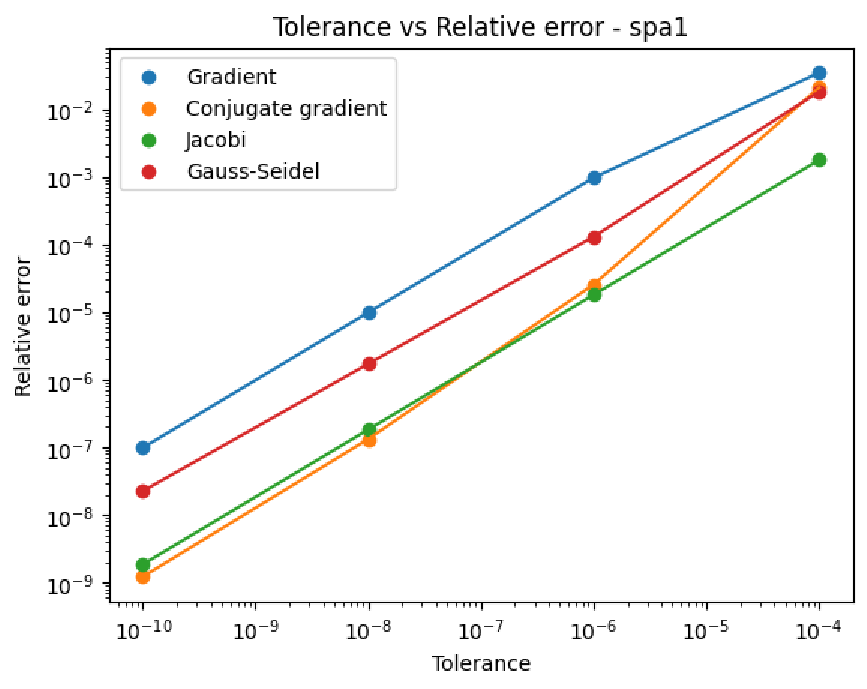
\includegraphics[width=0.40\textwidth]{figures/Tolerance vs Relative error/Difference between the 4 methods/spa1.pdf} }}%
	\subfloat{{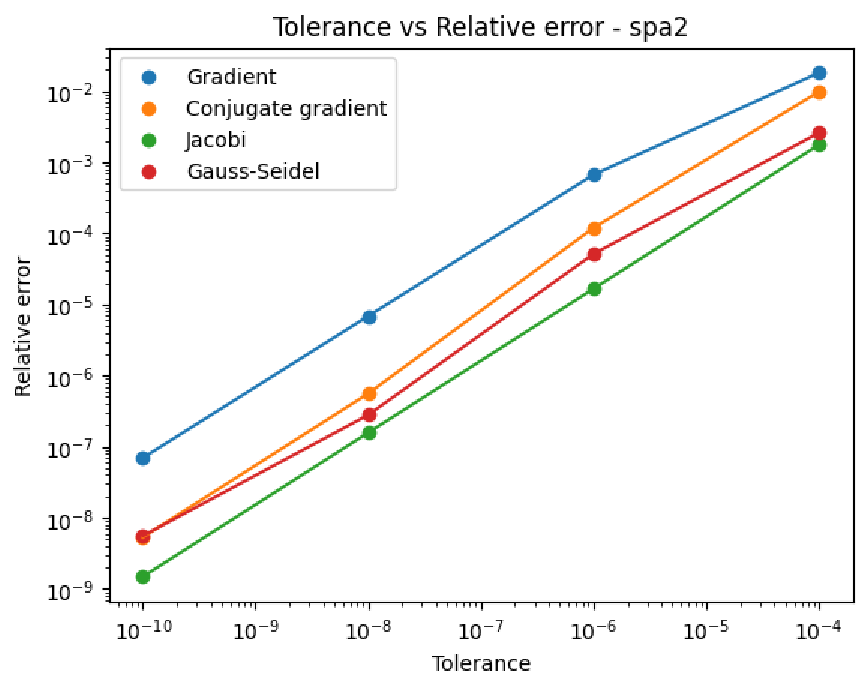
\includegraphics[width=0.40\textwidth]{figures/Tolerance vs Relative error/Difference between the 4 methods/spa2.pdf} }}%
	\qquad
	\subfloat{{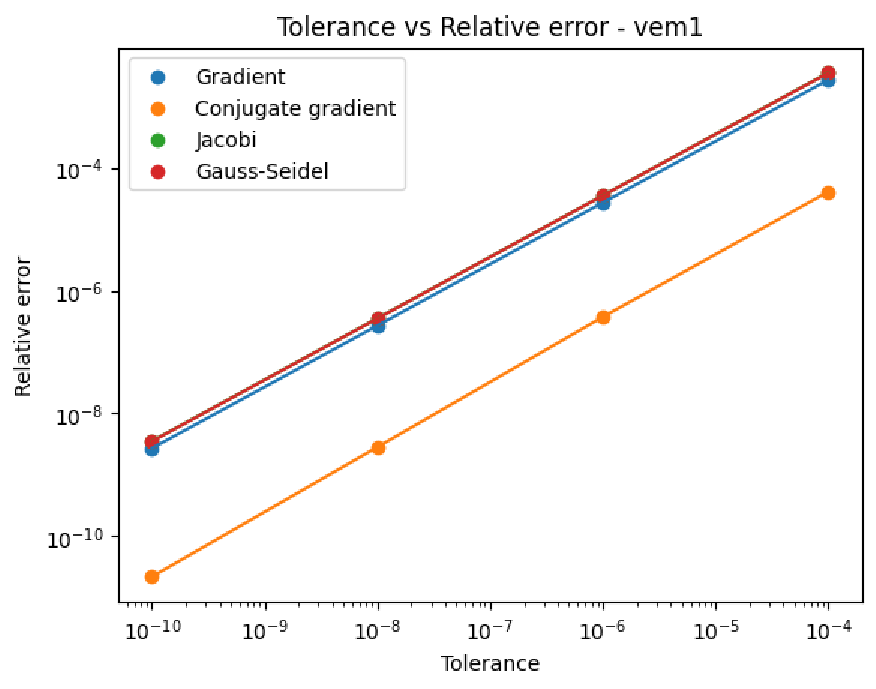
\includegraphics[width=0.40\textwidth]{figures/Tolerance vs Relative error/Difference between the 4 methods/vem1.pdf} }}%
	\subfloat{{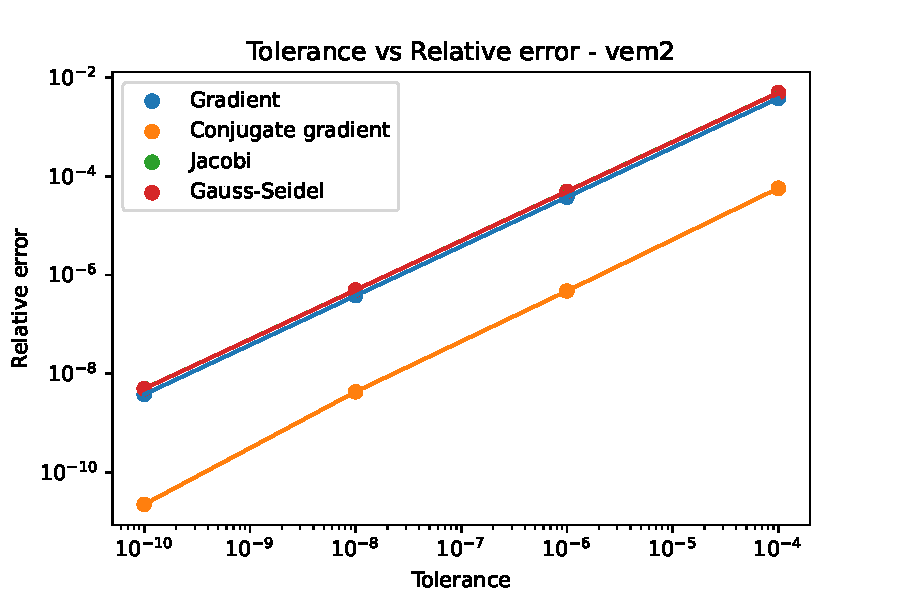
\includegraphics[width=0.40\textwidth]{figures/Tolerance vs Relative error/Difference between the 4 methods/vem2.pdf} }}%
	\caption{Grafici tolleranza / errore relativo sulle varie matrici di benchmark}%
	\label{fig:tolerrmat}
\end{figure}


\begin{figure}%
	\centering
	\subfloat{{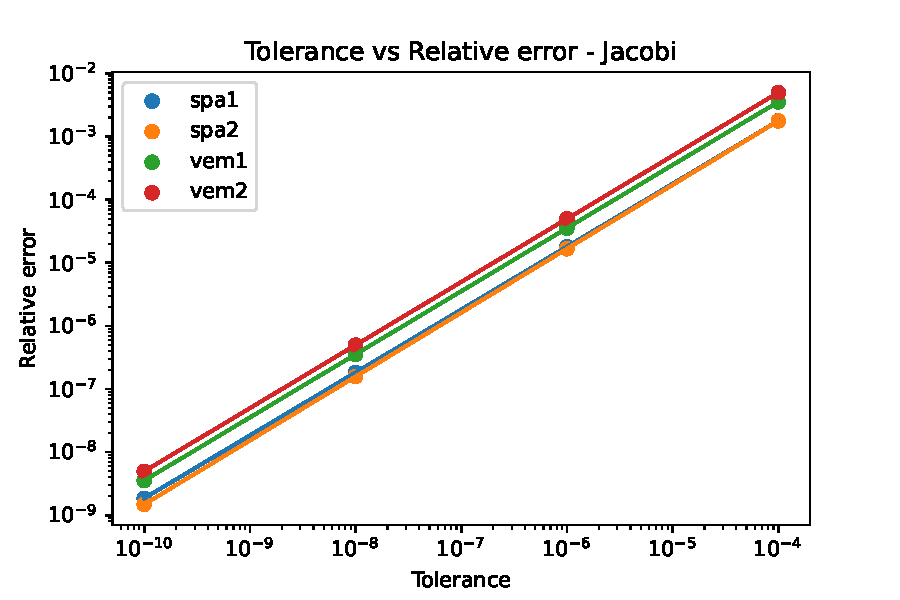
\includegraphics[width=0.40\textwidth]{figures/Tolerance vs Relative error/Difference between the 4 matrices on the same method/Jacobi.pdf} }}%
	\subfloat{{\includegraphics[width=0.40\textwidth]{figures/Tolerance vs Relative error/Difference between the 4 matrices on the same method/Conjugate Gradient.pdf} }}%
	\qquad
	\subfloat{{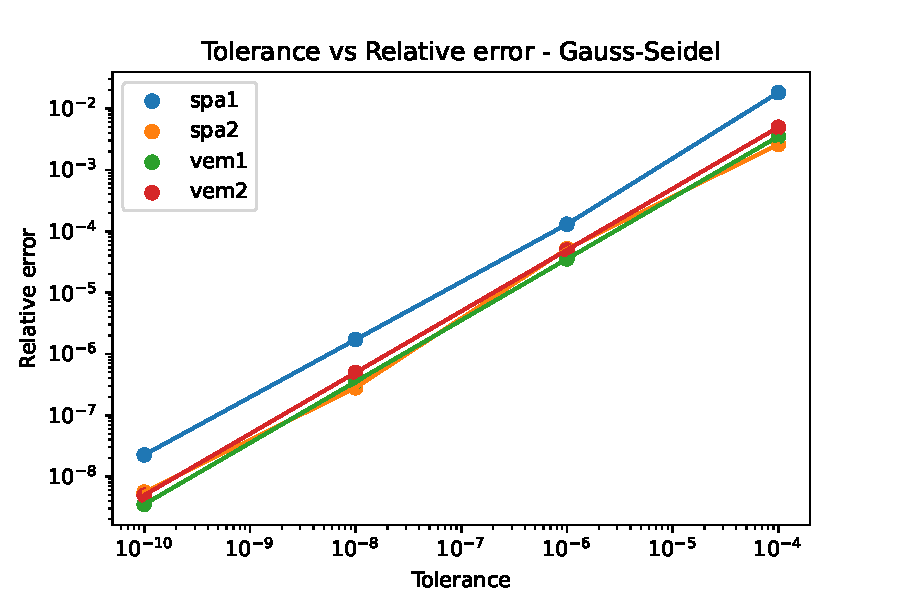
\includegraphics[width=0.40\textwidth]{figures/Tolerance vs Relative error/Difference between the 4 matrices on the same method/Gauss-Seidel.pdf} }}%
	\subfloat{{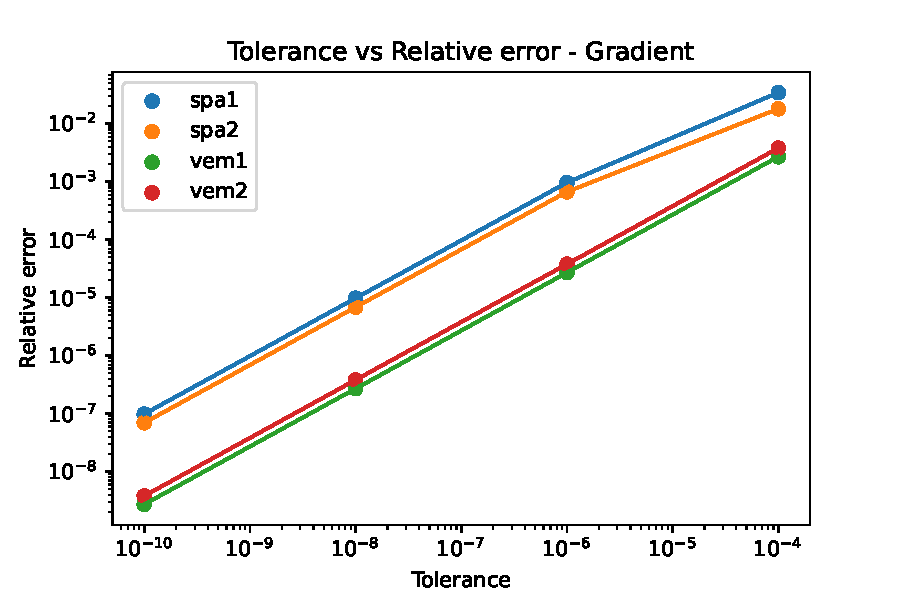
\includegraphics[width=0.40\textwidth]{figures/Tolerance vs Relative error/Difference between the 4 matrices on the same method/Gradient.pdf} }}%
	\caption{Grafici tolleranza / errore relativo rispetto i singoli metodi}%
	\label{fig:tolerrmet}
\end{figure}
%Immagine tolerance-relative_error, spa1, difference between the 4 methods
%Immagine tolerance-relative_error, spa2, difference between the 4 methods
%Immagine tolerance-relative_error, vem1, difference between the 4 methods
%Immagine tolerance-relative_error, vem2, difference between the 4 methods


Osservando i grafici che confrontano le matrici su singoli metodi, l'incremento dell'errore relativo sembra proporzionale alla crescita della tolleranza utilizzata durante l'esecuzione dei quattro metodi. Il risultato è ragionevole, così come indicato al capitolo \ref{tol/time, diff methods}, all'aumentare della tolleranza il criterio di arresto sarà meno restrittivo, portando ad una soluzione meno accurata, ergo ad un aumento dell'errore relativo. Quello che cambia, però, è il modo con cui l'errore cresce: infatti, sembra che i metodi con un valore più alto di errore, fissato un valore di tolleranza, siano anche quelli il cui errore cresce maggiomente alla diminuzione della tolleranza, considerato il fatto che la scala dei grafici è logaritmica.

Osservando, invece, i grafici che confrontano i risultati di ogni metodo sulle relative matrici, abbiamo notato che i metodi non stazionari hanno una particolare difficoltà a convergere verso la soluzione esatta nel caso delle matrici \texttt{spa1} e \texttt{spa2}; riteniamo che questa differenza più marcata in termini di errore relativo potrebbe essere dovuta al fatto che, probabilmente, i metodi basati su discesa del gradiente siano "avvantaggiati" nel trovare la strada giusta quando il numero di elementi non nulli è molto basso. Questo si può notare anche alla Figura \ref{fig:tolerrmat}, dove il metodo del gradiente coniugato manifesta un errore bassissimo rispetto agli altri e il metodo del gradiente "classico" resta comunque sotto i restanti due in termini di errori.

\paragraph{Tolleranza vs tempo trascorso}\label{tol/time, diff methods}


\begin{figure}%
	\centering
	\subfloat{{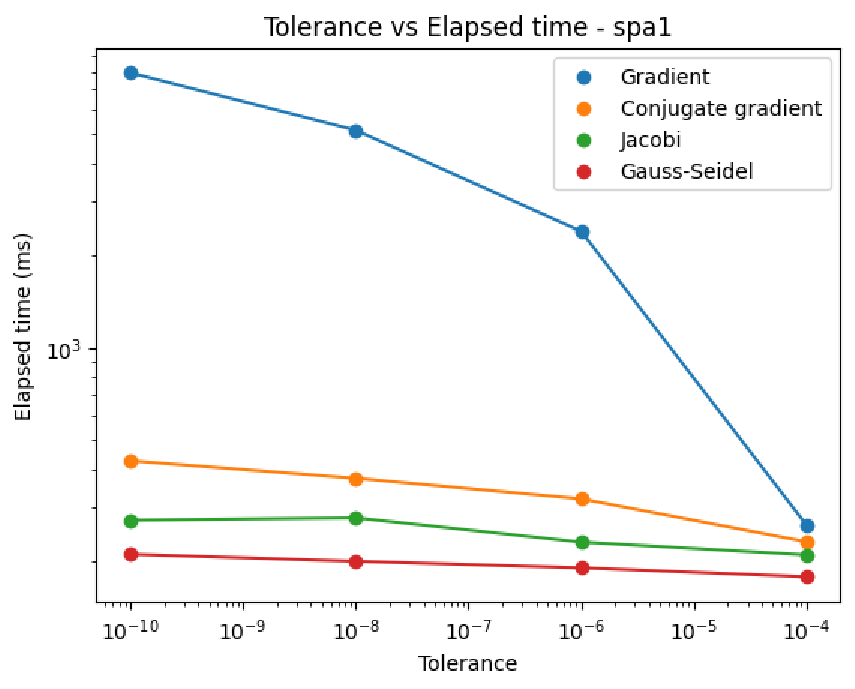
\includegraphics[width=0.40\textwidth]{figures/Tolerance vs Elapsed time/Difference between the 4 methods/spa1.pdf} }}%
	\subfloat{{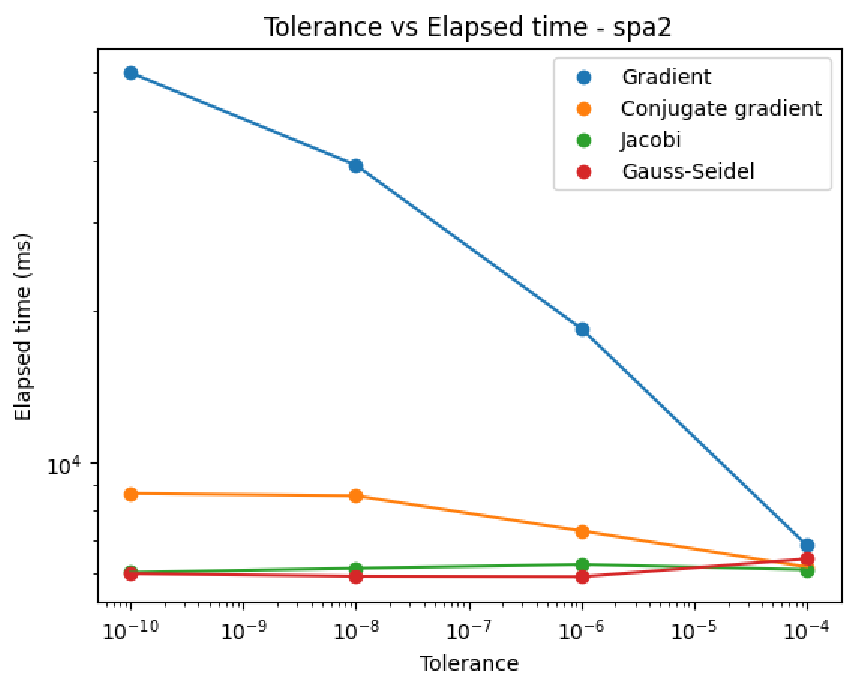
\includegraphics[width=0.40\textwidth]{figures/Tolerance vs Elapsed time/Difference between the 4 methods/spa2.pdf} }}%
	\qquad
	\subfloat{{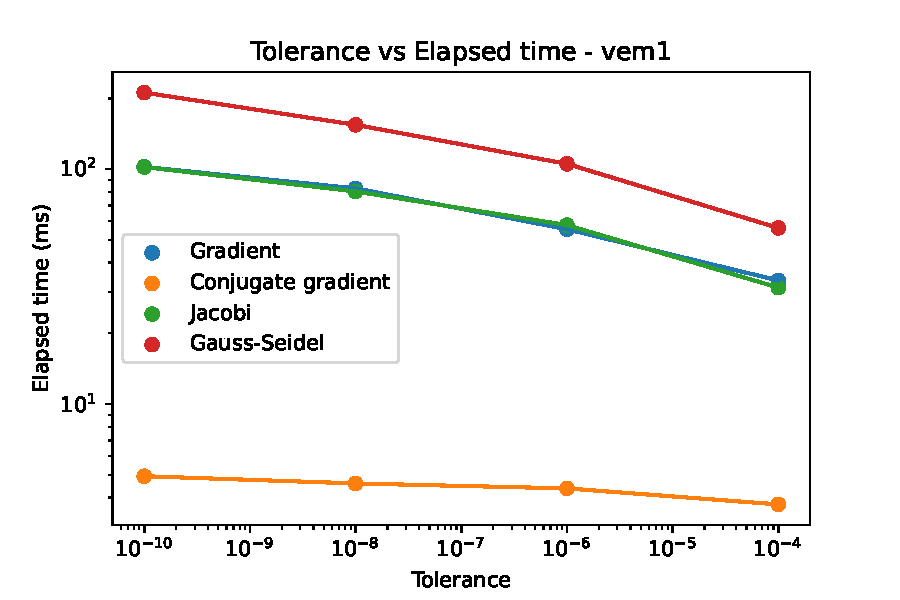
\includegraphics[width=0.40\textwidth]{figures/Tolerance vs Elapsed time/Difference between the 4 methods/vem1.pdf} }}%
	\subfloat{{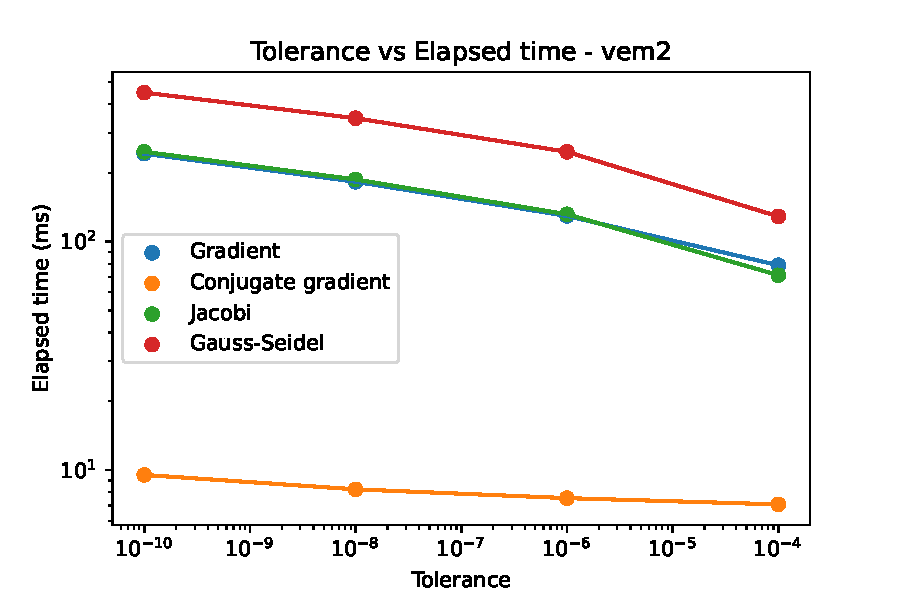
\includegraphics[width=0.40\textwidth]{figures/Tolerance vs Elapsed time/Difference between the 4 methods/vem2.pdf} }}%
	\caption{Grafici tolleranza / tempi sulle varie matrici di benchmark}%
	\label{fig:toltimemat}
\end{figure}

\begin{figure}%
	\centering
	\subfloat{{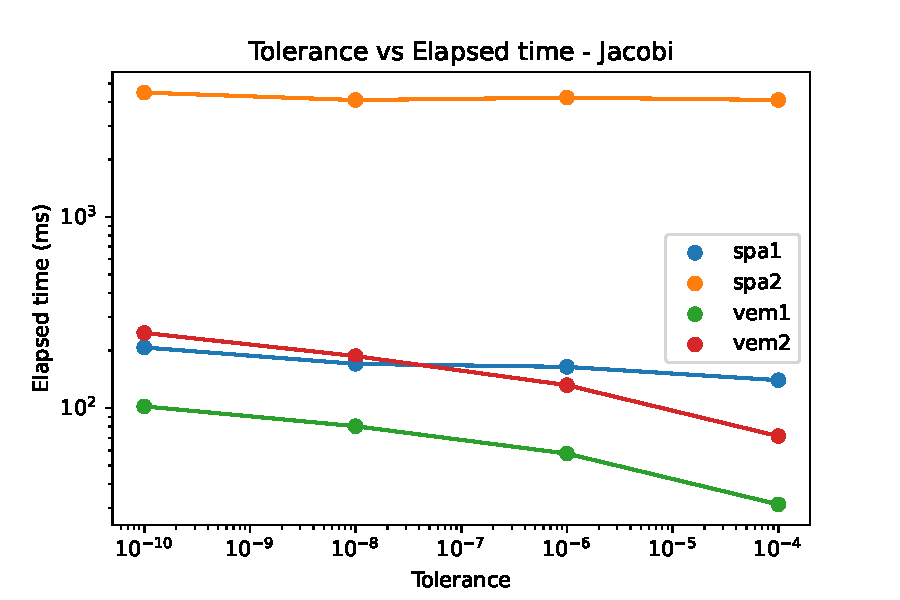
\includegraphics[width=0.40\textwidth]{figures/Tolerance vs Elapsed time/Difference between the 4 matrices on the same method/Jacobi.pdf} }}%
	\subfloat{{\includegraphics[width=0.40\textwidth]{figures/Tolerance vs Elapsed time/Difference between the 4 matrices on the same method/Conjugate Gradient.pdf} }}%
	\qquad
	\subfloat{{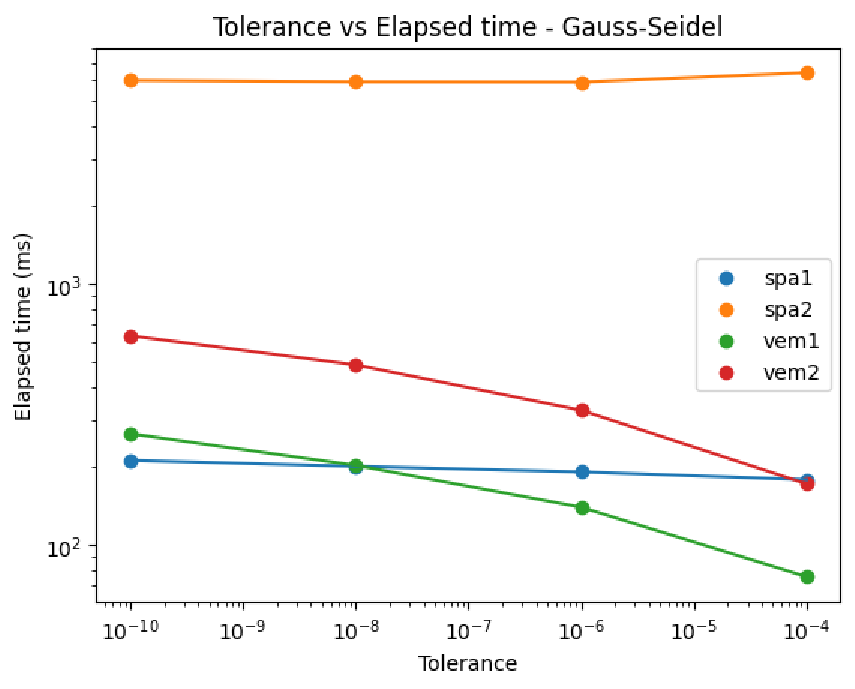
\includegraphics[width=0.40\textwidth]{figures/Tolerance vs Elapsed time/Difference between the 4 matrices on the same method/Gauss-Seidel.pdf} }}%
	\subfloat{{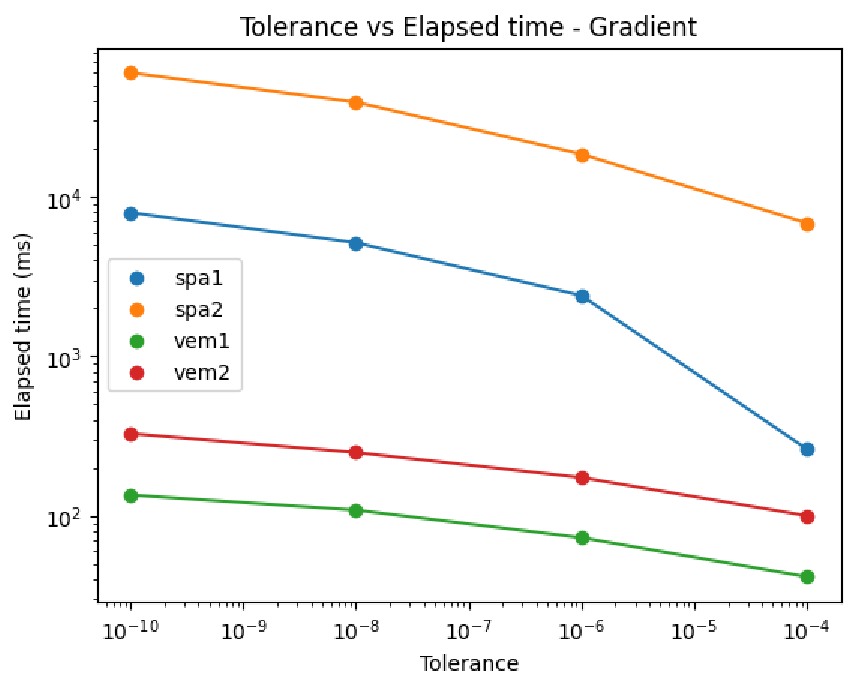
\includegraphics[width=0.40\textwidth]{figures/Tolerance vs Elapsed time/Difference between the 4 matrices on the same method/Gradient.pdf} }}%
	\caption{Grafici tolleranza / tempi rispetto i singoli metodi}%
	\label{fig:toltimemet}
\end{figure}
%Immagine tolerance-elapsedTime, spa1, difference between the 4 methods
%Immagine tolerance-elapsedTime, spa2, difference between the 4 methods

Nelle Figure \ref{fig:toltimemat} e \ref{fig:toltimemet} sono rappresentati i grafici relativi all'andamento del tempo rispetto alla tolleranza, raggruppati rispettivamente per matrice e per metodo.
Gauss Seidel è l'algoritmo che per le matrici relativamente dense, surclassa ogni altro metodo. Quando si passa a matrici estremamente sparse, come \path{vem1} e \path{vem2}, l'algoritmo che si comporta meglio sembra essere, invece, il gradiente coniugato. Questo è in accordo con ciò che abbiamo osservato in precedenza sugli errori, ovvero che i metodi non stazionari tendono a mostrare migliori prestazioni quando le matrici sono molto sparse.

Dai grafici si evince immediatamente che, all'aumentare della tolleranza, il tempo di esecuzione di ogni algoritmo tende a calare. Questa tendenza è più che ragionevole dato che, al calare della tolleranza, il criterio di arresto diventa più permissivo e l'algoritmo tenderà ad arrestarsi prima. Abbiamo notato, tuttavia, che ci sono metodi che sono molto più sensibili di altri in riferimento al tempo. Si può notare subito, ad esempio, il metodo del gradiente: il suo tempo di esecuzione, con la tolleranza minima, è di molto superiore a tutti gli altri; tuttavia, all'aumentare della tolleranza, il tempo scende in modo relativamente veloce, tendendo ad avvicinarsi alle prestazioni degli altri metodi. Questo tempo di esecuzione così alto è dovuto a un numero di iterazioni alto che, a sua volta, deriva, molto probabilmente, dalla difficoltà di avvicinarsi alla soluzione oltre a un certo limite di precisione.




